\documentclass{article}
% \usepackage[utf8]{inputenc}
\usepackage[backend=biber,citestyle=ieee]{biblatex}

\usepackage{pgfgantt}
\usepackage{graphicx}
\usepackage{xcolor}
\usepackage{float}
\usepackage{subfig}

% \usepackage{a4wide} 

\usepackage{fancyhdr}   %sidhuvud
\pagestyle{fancy}

\addbibresource{sources.bib}

\newcommand{\getauthor}{Oscar Fredriksson} %Author
\newcommand{\gettitle}{Visualization - Lab 1} %Title

\title{\gettitle}
\author{\getauthor}
\date{April 2021}

\begin{document}

    \pagenumbering{gobble}
    \maketitle

    \newpage

    \pagenumbering{arabic}

    \fancyhf{}
    \lhead{\getauthor}
    \rhead{\gettitle}
    \rfoot \thepage

    \section{First visualization}
    From the lecture and reading up on the internet it was evident that ISO-surfaces was a common way of visualizing volume. While exploring the Paraview filters the filter \textit{IsoVolume} was found which, after some tweaking gave a good representation of the teapot. The achieved visualization can be seen in figure \ref{fig:iso-volume}.

    % \begin{figure}[H]
    %     \centering
    %     \subfloat{{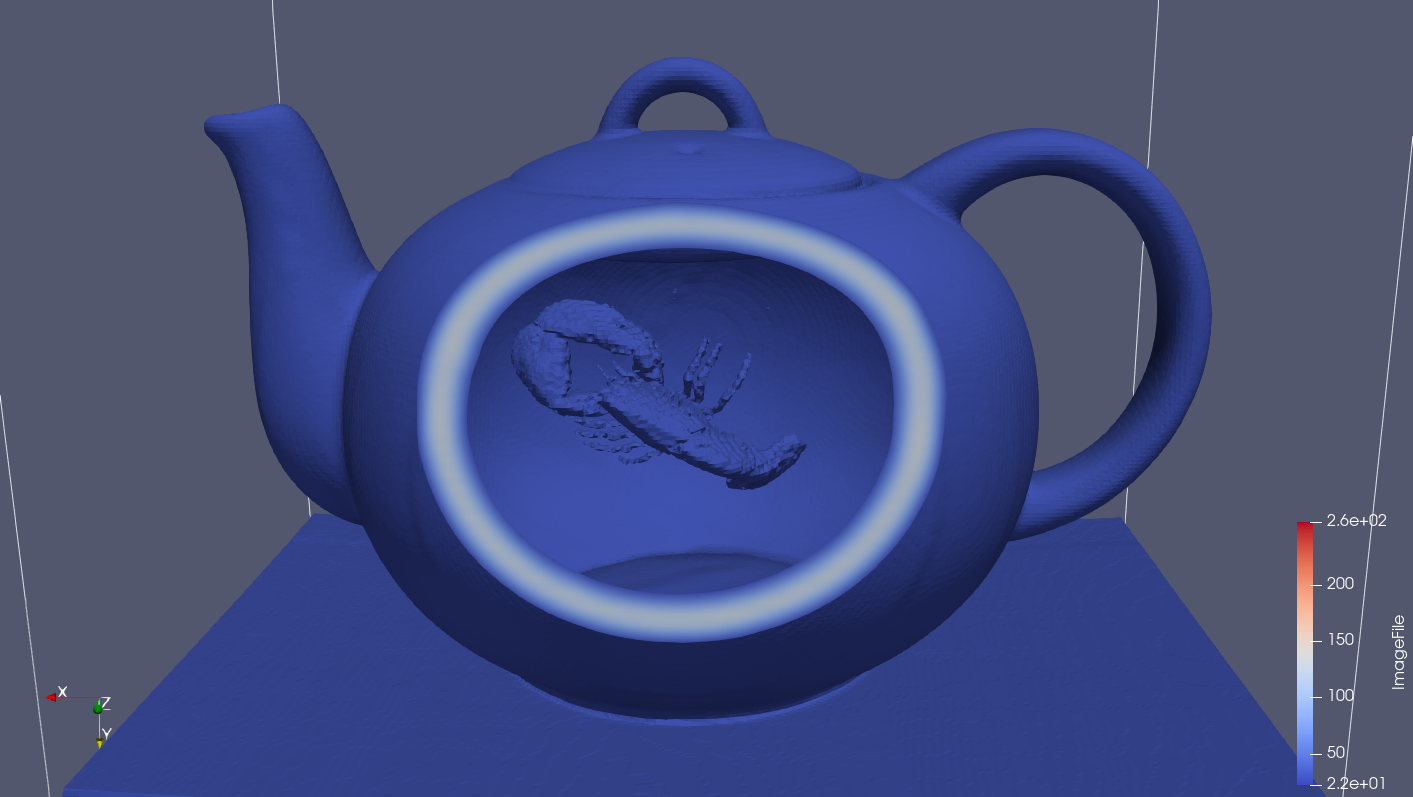
\includegraphics[width=0.46\textwidth]{img/teapot-iso-volume-clip.png} }}%
    %     \qquad
    %     \subfloat{{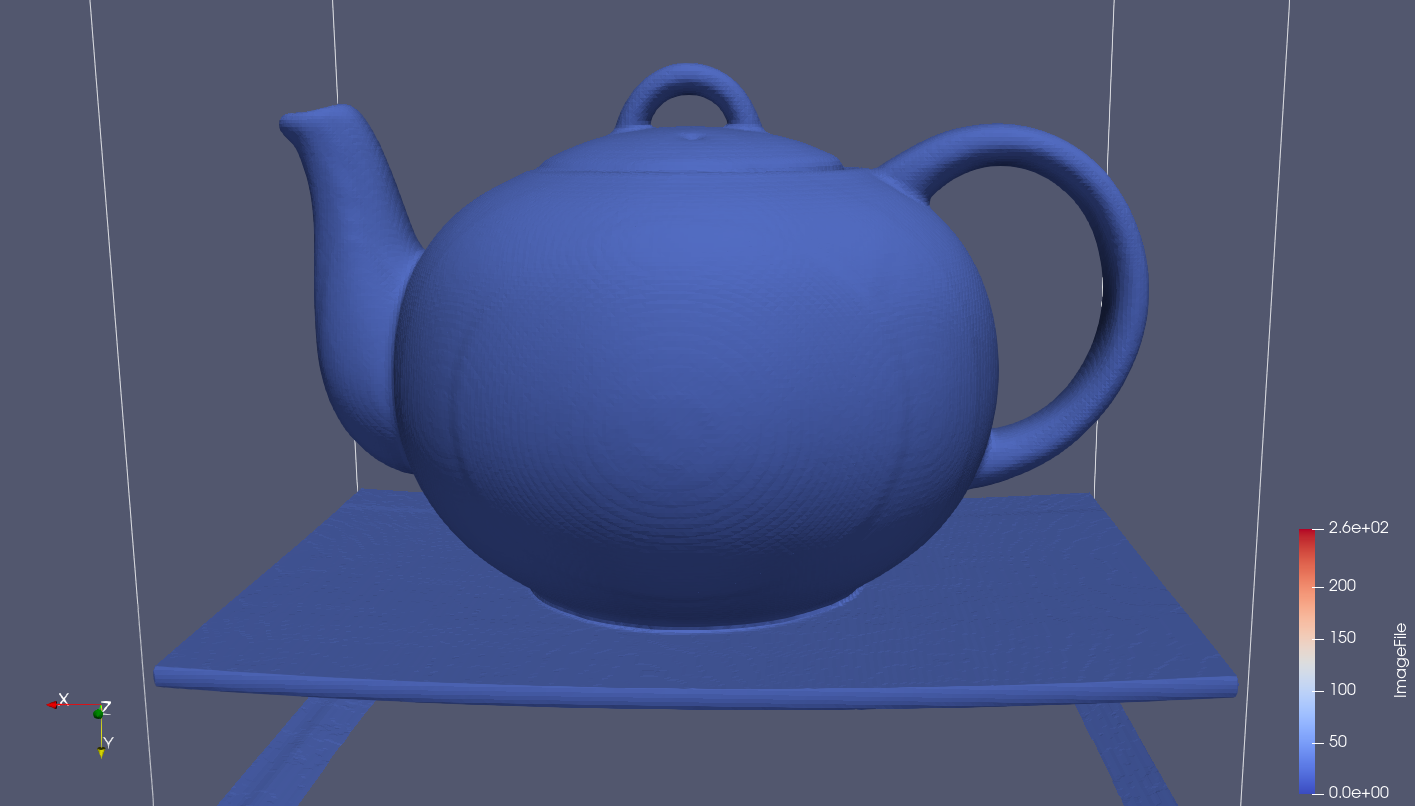
\includegraphics[width=0.46\textwidth]{img/teapot-iso-volume.png} }}%
        
    %     \caption{A visualization of the dataset using an iso-volume and clip.}
    %     \label{fig:visualization-1}
    %     \end{figure}

    \begin{figure}[H]
        \centering
        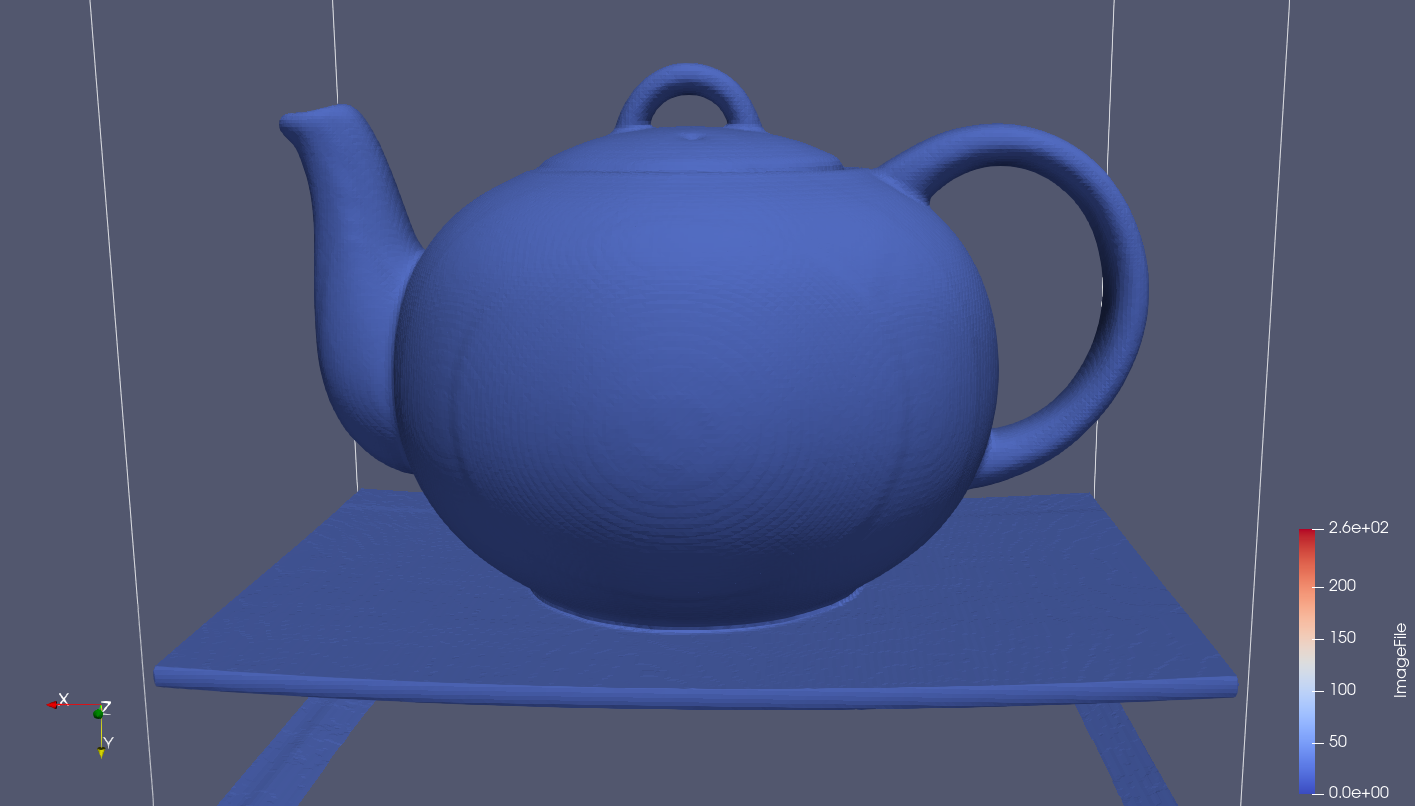
\includegraphics[width=0.6\textwidth]{img/teapot-iso-volume.png}
        
        \caption{A visualization of the dataset using an iso-volume.}
        \label{fig:iso-volume}
    \end{figure}

    After playing around with the opacity of the achieved surface it was discovered that the teapot contained a lobster. To visualize this without losing the teapot a \textit{Clip} filter was added

    \begin{figure}[H]
        \centering
        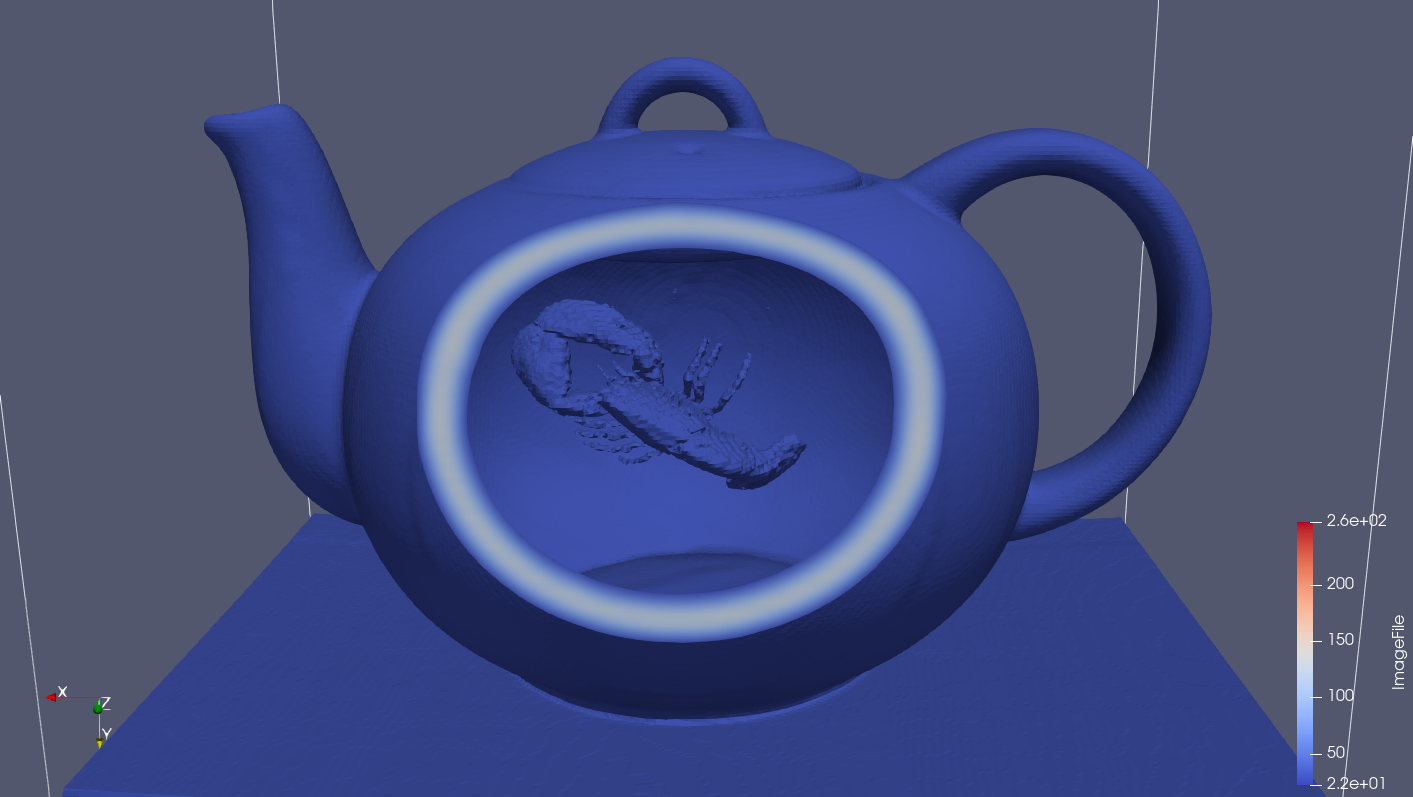
\includegraphics[width=0.6\textwidth]{img/teapot-iso-volume-clip.png}
        
        \caption{The same visualization as figure \ref{fig:iso-volume}, but with an added clip to see the lobster inside.}
        \label{fig:iso-volume-clip}
    \end{figure}

    \newpage
    % \printbibliography

\end{document}